\section{Measurement Model}
We consider the problem of recovery of a signal from its modulo measurements obtained through compressive sensing. Simply put, we aim to recover $\mathbf{x^*}\in \R^n$ from the modulo measurements $y_i=\mod(\langle \mathbf{a_i} \cdot \mathbf{x^*} \rangle,R)$ for $i = \{1,2,...,m\}$, where $\mod$ is modulo operation with respect to $R$. Typically, $m<n$. For simplicity, we assume that the modulo function operates only within two periods, one on the either side of the origin, as shown in the Fig.~\ref{fig:graph}. We construct $\mathbf{A} = \left[\mathbf{a_1~a_2~...~a_m}\right]^T$ with i.i.d. Gaussian entries. The primary assumption in our model is that the natural signal $\mathbf{x^*}$ is $s-$sparse in a chosen basis. 

\begin{figure}[h]
	\begin{center}
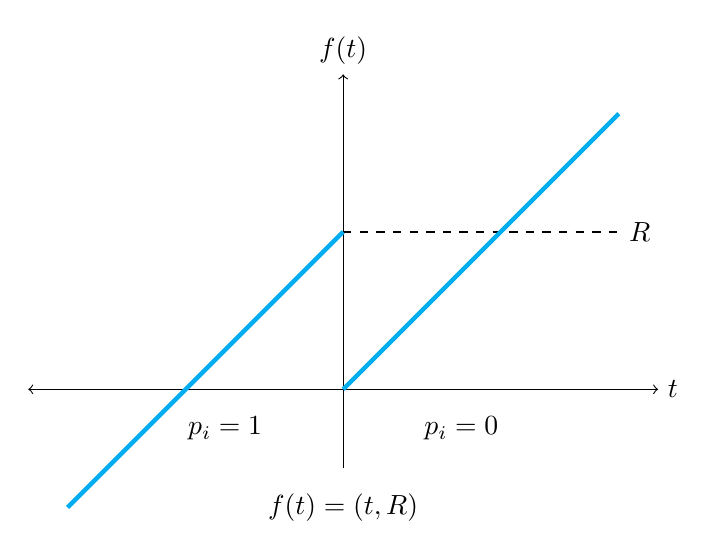
\begin{tikzpicture}
\draw[<->] (-4,0) -- (4,0) node[right] {$t$};
\draw[->] (0,-1) -- (0,4) node[above] {$f(t)$};
\draw[scale=0.5, dashed, thick] (0,4)--(7,4) node[right]{$R$};
\draw (1.5,-0.5) node(below) {$p_i = 0$};
\draw (-1.5,-0.5) node(below) {$p_i = 1$};
\draw (0,-1.5) node(right) {$f(t) = \mod(t,R)$};
\draw[scale=0.5,domain=-7:0,smooth,variable=\x,cyan, ultra thick] plot ({\x},{\x+4});
\draw[scale=0.5,domain=0:7,smooth,variable=\x,cyan, ultra thick]  plot ({\x},{\x});
\end{tikzpicture}
\end{center}
\caption{\emph{Modified modulo function for the given problem}}
\label{fig:graph}
\end{figure}

We can write the modified equation for the modulo operation under consideration as:
$$
\mathbf{y} = \mod(\mathbf{x^*},R) = \mathbf{x^*}+\left( \frac{1-\sgn(\mathbf{x^*})}{2}\right)R,
$$
where $\sgn(x)$ is a signum function.

We define the bin-index $p^*_i$ as,
$$
p^*_i = \frac{1-\sgn(\langle \mathbf{a_i} \cdot \mathbf{x^*} \rangle)}{2}.
$$
Thus,
$$
y_i = \langle \mathbf{a_i} \cdot \mathbf{x^*} \rangle + p^*_iR.
$$

It is evident that if we can recover $\mathbf{p^*}$ successfully, we can calculate the correct compressed measurements $\langle \mathbf{a_i} \cdot \mathbf{x^*} \rangle$ and use them to reconstruct $\mathbf{x^*}$ with any sparse recovery algorithm such as CoSaMP.


\section{Reconstruction Algorithm}

In this section, we describe our AltMin based approach to recover $\mathbf{x^*}$ and $\mathbf{p^*}$, given $\mathbf{y, A}, s, R$. We call our algorithm MoRAM - Modulo Reconstruction using Alternative Minimization.

We assume that we have access to an initial estimate of the signal $\mathbf{{x}^0}$ which is relatively close to the true vector $\mathbf{x^*}$. Starting with $\mathbf{{x}^0}$, we  calculate the estimates $\mathbf{p}$ and $\mathbf{x}$ in alternating fashion to converge to the original signal $\mathbf{x^*}$. At each iteration of our Alternative Minimization, we use the current estimate of the signal ${\mathbf{x^t}}$ to get the value of the bin-index vector $\mathbf{{p}^t}$ as following:
\begin{equation}
\mathbf{{p}^{t}} = \frac{\mathbf{1}-\sgn(\langle \mathbf{A} \cdot \mathbf{x^t} \rangle)}{2}.
\label{step1}
\end{equation}

 
 Given $\mathbf{x^0}$ is close to $\mathbf{x^*}$, $\mathbf{p^0}$ would also be close to $\mathbf{p^*}$. Ideal way is to calculate the correct compressed measurements $\mathbf{y^t_c}$ using $\mathbf{p^t}$, and use $\mathbf{y_c}$ with CoSaMP to calculate the next estimate $\mathbf{{x}_{t+1}}$. Thus,


$$
\mathbf{y^t_c} = \langle \mathbf{A}\mathbf{x_{t}} \rangle = \mathbf{y} - \mathbf{p^t}R,
$$
$$
\mathbf{{x}^{t+1}} = \argmin_{\mathbf{x} \in \mathcal{M}_s}\norm{\mathbf{Ax} - \mathbf{y^t_c}}_2^2, %~~\mathrm{s.to}~~x^* \in \mathcal{M}_s,
$$
$$
\implies \mathbf{{x}^{t+1}} = \cosamp(\frac{1}{\sqrt{m}}\mathbf{A},\frac{1}{\sqrt{m}}\mathbf{y^t_c},s,\mathbf{x_t}).
$$

 However, it should be noted that even the small error $\mathbf{d} = \mathbf{p^t - p^*}$ would reflect heavily in the calculation of $\mathbf{y^t_c}$, as each incorrect bin-index would add a noise of the magnitude $R$ in $\mathbf{y^t_c}$. Experiments suggest that the CoSaMP is not robust enough to cope up with such large errors in $\mathbf{y^t_c}$. To tackle this issue, we augmented the sparse recovery problem using the fact that the nature of error $\mathbf{d^t_p}$ is sparse; and each erroneous element of $\mathbf{p}$ adds a noise of the magnitude $R$ in $\mathbf{y^t_c}$. We take the sparsity of $\mathbf{d^t}$ to be $s_p = 0.1\times m$, suggesting that at most the $10\%$ of the total elements are classified with wrong bin-indices.
 
 The augmented optimization problem becomes,
  
$$
\mathbf{{x}^{t+1}}=\argmin_{[\mathbf{x~d}]^T \in \mathcal{M}_{s+s_p}}\norm{\begin{bmatrix} \mathbf{A} & \mathbf{I} \end{bmatrix} \begin{bmatrix} \mathbf{x} \\ \mathbf{d} \end{bmatrix} - \mathbf{y}}_2^2, %~~\mathrm{s.to}~~x^* \in \mathcal{M}_s,
$$
\begin{equation}
\implies \mathbf{{x^{t+1}}} = \cosamp(\frac{1}{\sqrt{m}}\begin{bmatrix} \mathbf{A} & \mathbf{I} \end{bmatrix},\frac{1}{\sqrt{m}}\mathbf{y},s+s_p,[\mathbf{x^t~~p^t}]^T).
\label{step2}
\end{equation}
We repeat the steps as in Eq.~\ref{step1} and Eq.~\ref{step2} alternatively for $\mathrm{N}$ iterations. 

%$$
%\norm{\begin{bmatrix} \mathbf{A} & \mathbf{I} \end{bmatrix} \begin{bmatrix} \mathbf{x^*} \\ \mathbf{d} \end{bmatrix} - \mathbf{y}}_2^2.
%$$

%
\begin{algorithm}[t]
	\caption{\textsc{MoRAM}}
	\label{alg:DMF}
	\begin{algorithmic}
		\State\textbf{Inputs:} $\mathbf{y}$, $\mathbf{A}$, $s$, $R$
		\State\textbf{Output:}  $\widehat{x}$
		\State $m,n \leftarrow \mathrm{size}(\mathbf{A})$ 
		\State $s_p \leftarrow 0.1\cdot m$
		\State \textbf{Initialization}
		\State $\mathbf{x^0} \leftarrow \textrm{Oracle}(\mathbf{y, A})$ 
		\State \textbf{Alternative Minimization}
		\For {$l =0:\mathrm{N}$}
		\State $\mathbf{{p}^{t}} \leftarrow \frac{\mathbf{1}-\sgn(\langle \mathbf{A} \cdot \mathbf{x^t} \rangle)}{2}$
		\State $\mathbf{{x}^{t+1}}\leftarrow \argmin_{[\mathbf{x~d}]^T \in \mathcal{M}_{s+s_p}}\norm{\begin{bmatrix} \mathbf{A} & \mathbf{I} \end{bmatrix} \begin{bmatrix} \mathbf{x} \\ \mathbf{d} \end{bmatrix} - \mathbf{y}}_2^2 = \cosamp(\frac{1}{\sqrt{m}}\begin{bmatrix} \mathbf{A} & \mathbf{I} \end{bmatrix},\frac{1}{\sqrt{m}}\mathbf{y},s+s_p,[\mathbf{x^t~~p^t}]^T)$
		\EndFor
	\end{algorithmic}
\end{algorithm}



\subsection{Experiments}
We test our algorithm on a synthetic signal generated randomly with $n=1000$ and $s=20$. 

Our aim is to analyze the sensitivity of our algorithm towards the initial estimate $\mathbf{x^0}$. %Currently, in the absence of a suitable initialization method, 
For that, we compute the initial estimate $\mathbf{x^0}$ by adding a Gaussian noise to the original signal. In Fig.~\ref{fig:pl}, we plot the variation of the relative reconstruction error ($\frac{\norm{\mathbf{x^*-x^N}}}{\norm{\mathbf{x^*}}}$) with the relative error in initial estimate ($\frac{\norm{\mathbf{x^*-x^0}}}{\norm{\mathbf{x^*}}}$). We plot the similar curves for different values of number of measurements $m$.
\begin{figure}[t]
	\begin{center}
		%\vspace{-0em}
		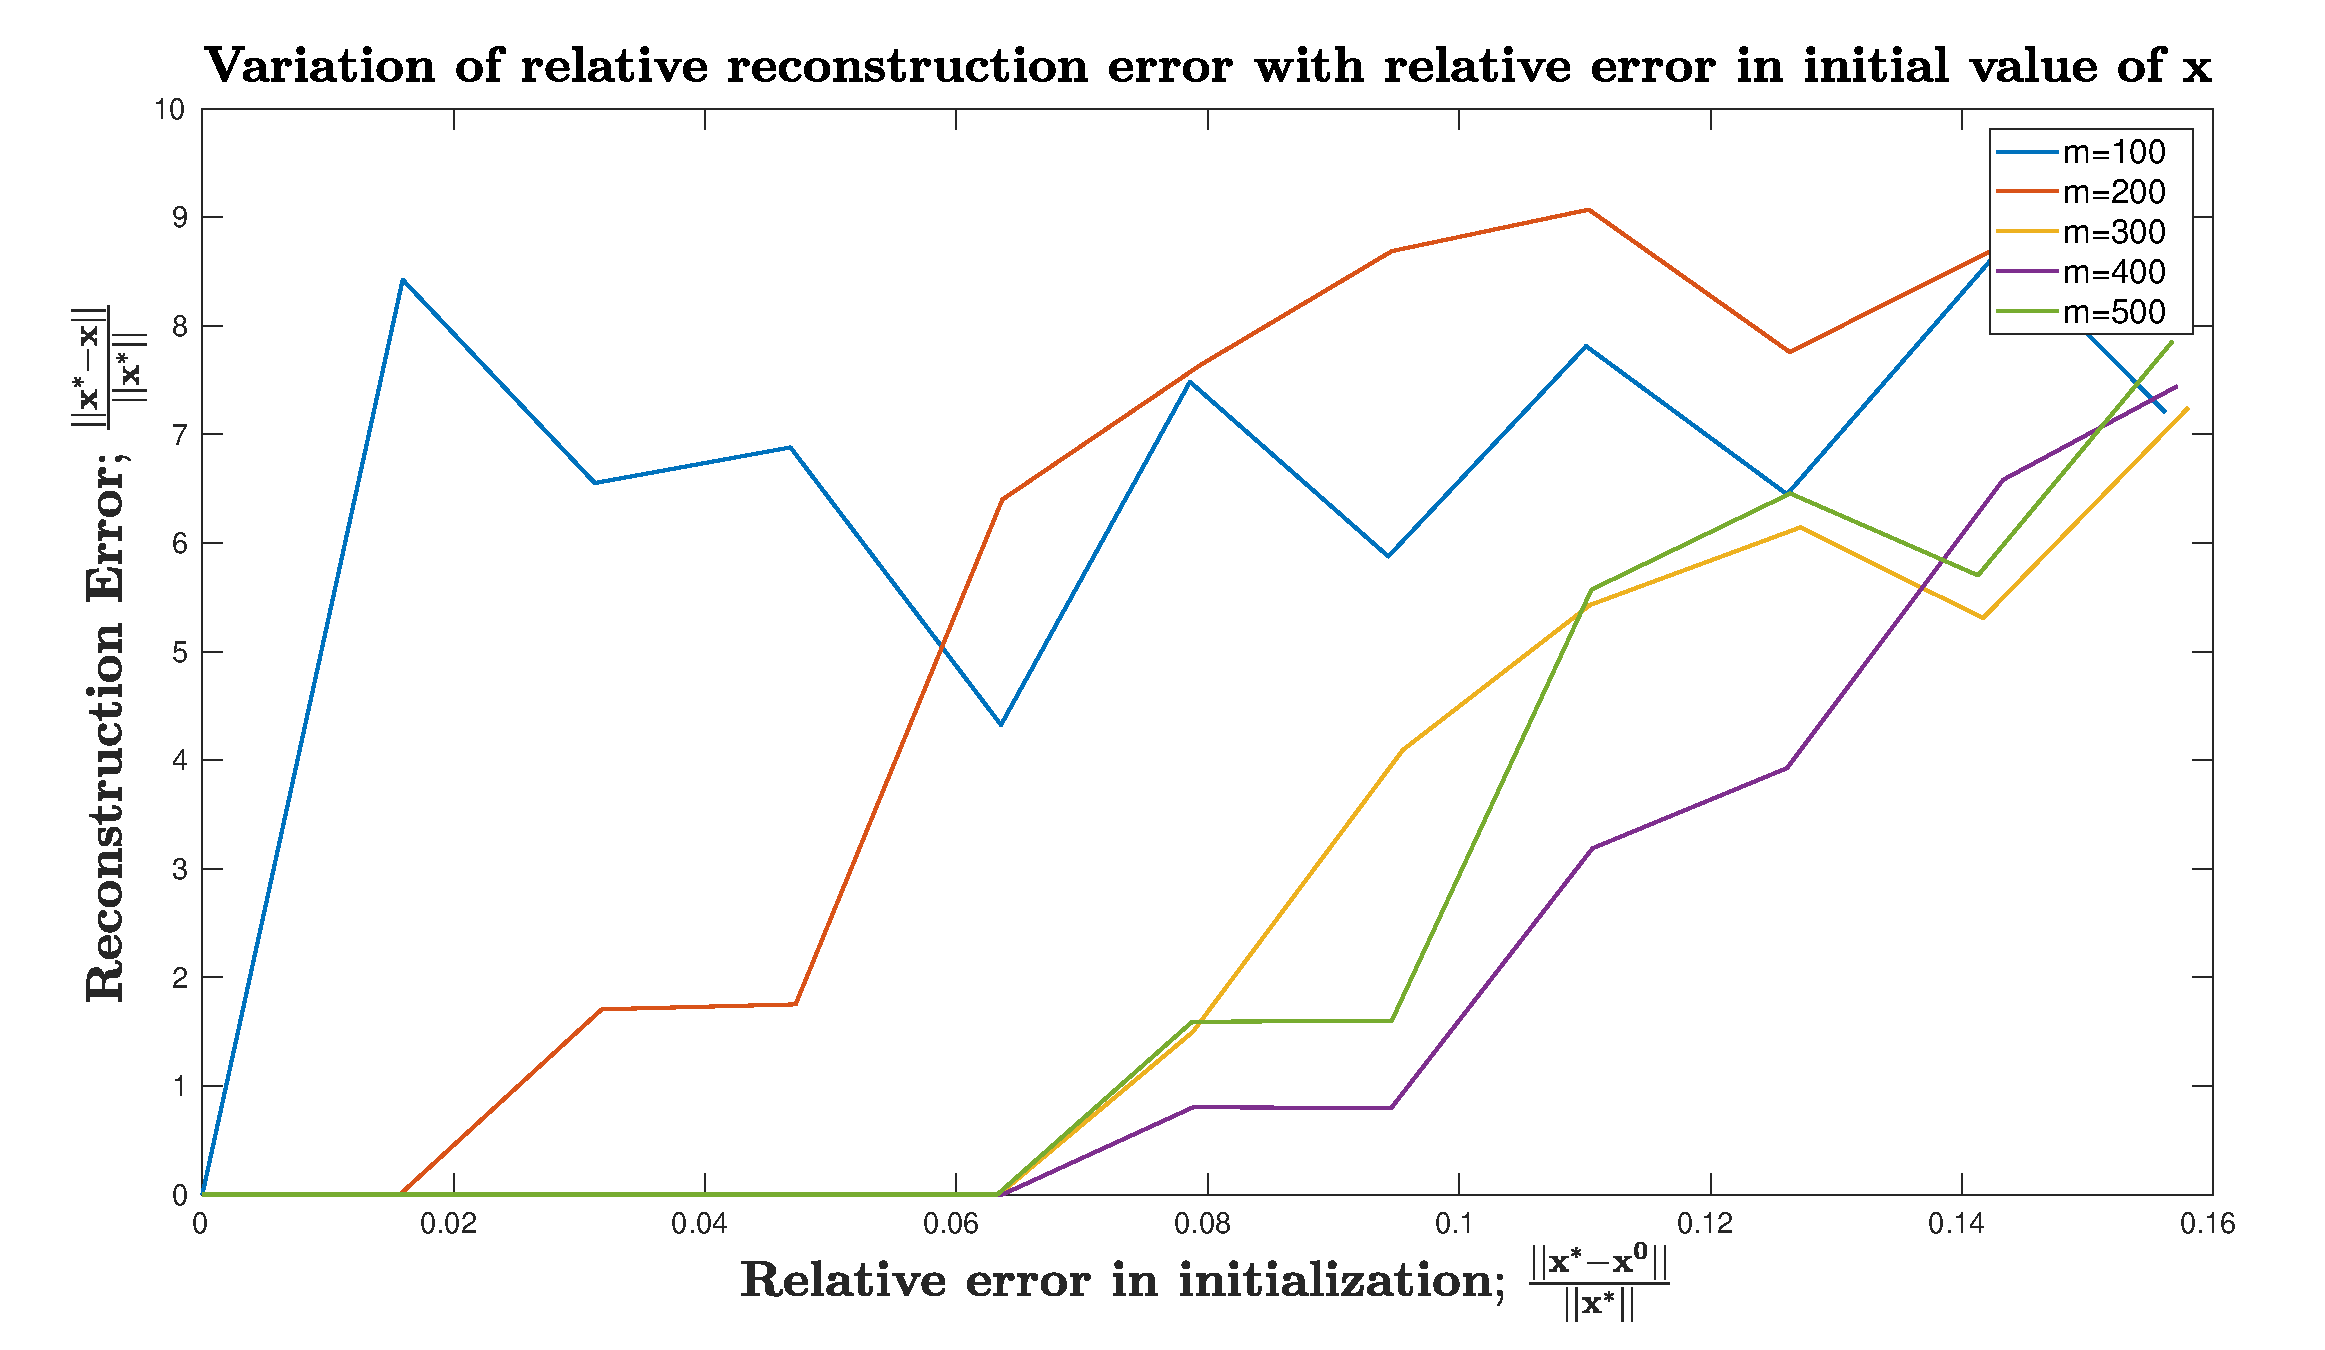
\includegraphics[width=\linewidth]{./fig/graph.pdf}
	\end{center}
	\caption{}
	\label{fig:pl}
\end{figure}

%\newpage
%\begin{section}{Appendix}
%\begin{figure}[t]
%	\begin{center}
%		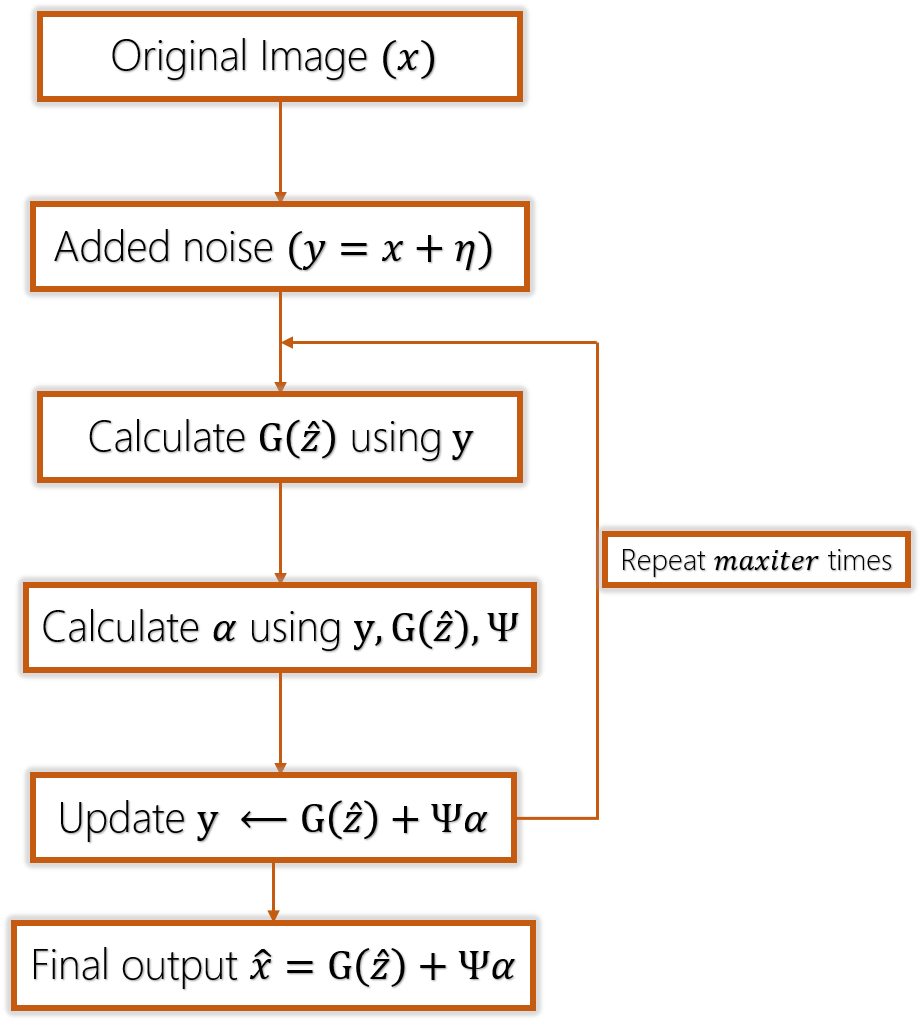
\includegraphics[width=0.4\linewidth]{./fig/alg.png}
%	\end{center}
%	\caption{\emph{Our approach}}
%	\label{fig:alg}
%\end{figure}
%\end{section}
